\chapter{Wprowadzenie do IoT i związanych z nim zagrożeń}
\label{chap:rozdzial2}  
\section{Wprowadzenie do tematyki IoT}
\textbf{Internet Rzeczy (IoT - Internet of Things)} to koncepcja sieciowej komunikacji między fizycznymi urządzeniami wyposażonymi w sensory, oprogramowanie i technologie łączności, umożliwiająca im gromadzenie, przetwarzanie i wymianę danych. W przeciwieństwie do tradycyjnego internetu, który skupia się na wymianie informacji między ludźmi, IoT tworzy rozproszony ekosystem, w którym przedmioty („rzeczy”) autonomicznie współdziałają ze sobą, z infrastrukturą chmurową oraz z systemami nadrzędnymi poprzez sieci przewodowe i bezprzewodowe. Ogólną strukturę takiego systemu przedstawiono na rysunku \ref{fig:Trzy główne elementy IoT}.
\vspace{1cm}\\
\textbf{Kluczowe cechy IoT}
    \begin{itemize}
        \item \textbf{Autonomiczność} - Urządzenia IoT dzięki wbudowanym mechanizmom mogą analizować dane środowiskowe, wykrywać anomalie i podejmować złożone decyzje (np. regulacja parametrów procesów przemysłowych) bez stałego nadzoru człowieka. Przykładem są inteligentne systemy zarządzania energią, które optymalizują pobór mocy w czasie rzeczywistym.
        \item \textbf{Komunikacja M2M} (Machine-to-Machine) - Wymiana informacji między urządzeniami (np. między czujnikami temperatury a systemem klimatyzacji w smart building) odbywa się poprzez standardowe protokoły (MQTT, CoAP, LoRaWAN) bez konieczności interwencji użytkownika \cite{IEEE2413}.
        \item \textbf{Heterogeniczność } - Różnorodność urządzeń (od prostych sensorów po zaawansowane roboty przemysłowe), wieloprotokołowość (komunikacja poprzez różne protokoły w zależności od wymagań energetycznych i przepustowości) oraz różne systemy operacyjne (RIOT, FreeRTOS, Linux) i platformy chmurowe (AWS IoT, Azure Sphere).
        \item \textbf{Integracja z chmurą i edge computing} - Przetwarzanie danych odbywa się hierarchicznie w warstwie brzegowej (lokalna analiza danych na urządzeniach wejściowych w celu redukcji opóźnień), chmurze (agregacja danych z wielu źródeł i zaawansowana analityka np. predykcyjne utrzymanie ruchu w IIoT), czy hybrydowe modele fog computing (przetwarzanie wrażliwych danych medycznych w lokalnej chmurze z zachowaniem zgodności prawnej (GDRP/HIPAA)) \cite{bonomi2012fog}.
    \end{itemize}

\begin{figure}[h]
    \centering
    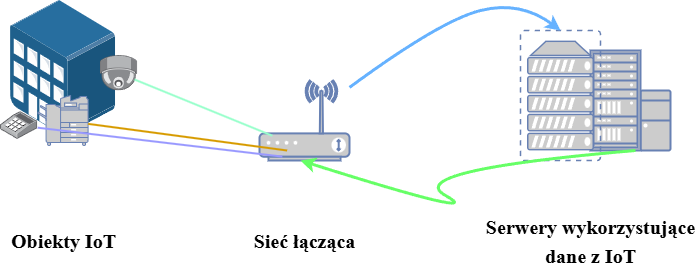
\includegraphics[width=0.8\textwidth]{pictures/IoT_basic.drawio.png}
    \caption{Trzy główne elementy IoT}
    \label{fig:Trzy główne elementy IoT}
\end{figure}

\vspace{1cm}

\textbf{Znaczenie IoT w różnych dziedzinach życia i gospodarki}
    \begin{itemize}
    \item \textbf{Gospodarka i Przemysł 4.0} – Internet Rzeczy jest kluczowym elementem transformacji cyfrowej przemysłu, znanej jako Przemysł 4.0. Dzięki integracji czujników i urządzeń z systemami produkcyjnymi możliwa jest ciągła analiza danych z maszyn, co pozwala przewidywać awarie, automatyzować linie produkcyjne oraz dynamicznie zarządzać zasobami. To z kolei przekłada się na zwiększenie wydajności, redukcję kosztów oraz poprawę jakości produktów.

    \item \textbf{Opieka zdrowotna} – IoT rewolucjonizuje sektor medyczny, umożliwiając zdalne monitorowanie pacjentów w czasie rzeczywistym, niezależnie od ich lokalizacji. Urządzenia noszone (np. smartwatche, inteligentne opaski) monitorują tętno, ciśnienie krwi, poziom cukru i inne parametry, przesyłając dane bezpośrednio do systemów lekarzy. Taka technologia znacząco zwiększa skuteczność leczenia przewlekłych chorób, poprawia jakość życia pacjentów oraz odciąża systemy opieki zdrowotnej.

    \item \textbf{Inteligentne miasta (Smart Cities)} – IoT umożliwia efektywne zarządzanie przestrzenią miejską i usługami publicznymi. Przykładowo, inteligentne systemy zarządzania ruchem drogowym pozwalają zmniejszyć korki i emisję spalin, a czujniki jakości powietrza umożliwiają monitorowanie poziomu zanieczyszczeń w czasie rzeczywistym. Oświetlenie uliczne może automatycznie dostosowywać natężenie światła w zależności od ruchu, co zmniejsza zużycie energii. Dzięki IoT miasta stają się bardziej przyjazne mieszkańcom, zrównoważone i nowoczesne.

    \item \textbf{Inteligentne domy (Smart Homes)} – W sferze prywatnej IoT zapewnia wygodę i bezpieczeństwo. Użytkownicy mogą zdalnie sterować systemami ogrzewania, klimatyzacji, oświetlenia czy domowymi urządzeniami elektronicznymi za pomocą smartfonów lub asystentów głosowych. Inteligentne zamki, alarmy i kamery zwiększają poziom ochrony, a automatyzacja procesów (np. harmonogramy włączania urządzeń) prowadzi do oszczędności energii i niższych rachunków.

    \item \textbf{Transport i logistyka} – Dzięki IoT firmy transportowe i logistyczne mogą śledzić pojazdy, monitorować warunki transportu (np. temperaturę w chłodniach), przewidywać opóźnienia oraz optymalizować trasy w czasie rzeczywistym. Technologie takie jak RFID i GPS w połączeniu z platformami analitycznymi pozwalają na dokładniejsze zarządzanie łańcuchem dostaw, redukując straty i zwiększając niezawodność dostaw.

    \item \textbf{Rolnictwo (Smart Agriculture)} – IoT ma ogromny potencjał w rolnictwie precyzyjnym. Czujniki gleby, stacje pogodowe i drony umożliwiają rolnikom monitorowanie warunków środowiskowych i upraw, automatyzację nawadniania czy kontrolę nad nawożeniem. Dzięki temu możliwe jest zwiększenie plonów, zmniejszenie zużycia wody i środków chemicznych oraz ograniczenie wpływu na środowisko. Systemy te wspierają także monitorowanie stanu zdrowia zwierząt hodowlanych, co przekłada się na lepszą jakość i efektywność produkcji \cite{wolfert2017big}.
\end{itemize}

\section{Kluczowe pojęcia związane z prywatnością i bezpieczeństwem danych w IoT}
\textbf{Prywatność} w systemach IoT odnosi się do ochrony danych osobowych użytkowników, ich anonimowości oraz metadanych zbieranych przez urządzenia IoT. W kontekście IoT prywatność zyskuje szczególne znaczenie, ponieważ urządzenia te często gromadzą bardzo wrażliwe informacje — na przykład dane zdrowotne, lokalizacyjne, czy osobiste preferencje użytkowników. Ponieważ wiele urządzeń łączy się z chmurą i innymi systemami w sieci, zagrożenia związane z niewłaściwym zarządzaniem tymi danymi są wysokie.

W praktyce zapewnienie prywatności oznacza wdrożenie odpowiednich polityk ochrony danych, takich jak zgodność z regulacjami prawnymi (np. RODO w Europie). Ważne jest stosowanie mechanizmów szyfrowania danych zarówno podczas transmisji, jak i ich przechowywania, aby uniemożliwić dostęp osobom nieuprawnionym. Równie istotna jest transparentność wobec użytkowników — powinni oni być informowani, jakie dane są zbierane, w jaki sposób są wykorzystywane i komu mogą być udostępniane. Ponadto, użytkownicy powinni mieć realną kontrolę nad swoimi danymi, np. możliwość ich usunięcia lub zmiany zgód na przetwarzanie.

\textbf{Bezpieczeństwo} danych w systemach IoT to szeroki zakres działań mających na celu ochronę integralności, poufności oraz dostępności informacji. Ze względu na rozproszoną architekturę IoT i ogromną liczbę połączonych urządzeń, systemy te są szczególnie podatne na różnorodne ataki. Do najczęstszych należą: manipulacja danymi, nieautoryzowany dostęp do urządzeń i sieci, ataki DDoS (Distributed Denial of Service), które przeciążają systemy, a także wstrzykiwanie złośliwego oprogramowania (malware), które może przejąć kontrolę nad urządzeniem lub całym systemem.

Aby przeciwdziałać tym zagrożeniom, kluczowe jest stosowanie zaawansowanych mechanizmów ochrony, takich jak:
\begin{itemize}
    \item \textbf{Szyfrowanie} - Zabezpieczenie danych przed przechwyceniem i odczytaniem.

    \item \textbf{Uwierzytelnianie} - Weryfikacja tożsamości urządzeń i użytkowników.
    
    \item \textbf{Zarządzanie tożsamościami i uprawnieniami} - Nadawanie odpowiednich ról i dostępów.
    
    \item \textbf{Monitorowanie i wykrywanie zagrożeń } - Ciągłe śledzenie zachowań w sieci i szybkie reagowanie na anomalie.
\end{itemize}

\textbf{Protokoły komunikuacyjne w systemach IoT} odgrywają kluczową rolę, umożliwiając urządzeniom wymianę danych i współpracę w sieci. Protokoły te są lekkie i energooszczędne, dostosowane do ograniczonych zasobów urządzeń. Można wyróżnić kilka kluczowych protokołów, takich jak: MQTT, CoAP, BLE, LoRaWAN.

\section{Różnorodność urządzeń IoT}
Systemy IoT integrują heterogeniczne urządzenia, które można sklasyfikować według dwóch kluczowych kryteriów:

\subsubsection{Klasyfikacja według zasobów obliczeniowych:}
    \begin{enumerate}
        \item \textbf{Urządzenia wysokiej mocy}: \\
        Urządzenia tego typu dysponują dużą mocą obliczeniową, często posiadają własne systemy operacyjne, wsparcie dla wielu protokołów komunikacyjnych i są zdolne do lokalnego przetwarzania danych bez konieczności stałego połączenia z chmurą.
        \begin{itemize}
            \item \textbf{Przykłady}: Roboty przemysłowe, serwery brzegowe (edge servers), bramki IoT (gateway), systemy SCADA (Supervisory Control and Data Acquisition), systemy MES (Manufacturing Execution Systems), sterowniki PLC (Programmable Logic Controllers). 
            \item \textbf{Zastosowania}: Lokalna analiza danych w czasie rzeczywistym (edge computing), agregacja danych z wielu czujników i ich przesyłanie do chmury, sterowanie złożonymi procesami przemysłowymi, reakcja na krytyczne zdarzenia bez opóźnień związanych z przesyłem do chmury.
            \item \textbf{Wyzwania bezpieczeństwa}: Ataki na interfejsy i protokoły (na podatne API lub niezabezpieczone porty), luki w aktualizacjach oprogramowania (brak automatycznych aktualizacji), ataki DDoS/DoS (przeciążenie bramki lub serwera brzegowego), złośliwe oprogramowanie.
        \end{itemize}
        \item \textbf{Urządzenia ograniczone zasobowo}: \\
        To małe, często jednozadaniowe urządzenia, które charakteryzują się niskim poborem mocy i ograniczoną pamięcią oraz mocą obliczeniową.
        \begin{itemize}
            \item \textbf{Przykłady}: Czujniki temperatury, wilgotności, ruchu, tagi RFID, urządzenia noszone (wearables), smartwatche, pompy insulinowe, inteligentne zamki, inteligentne termostaty. Zbieranie danych z otoczenia (np. środowiska, biometrycznych), identyfikacja i śledzenie (np. za pomocą RFID), zarządzanie energią i zużyciem w budynkach (smart building), monitorowanie stanu zdrowia w czasie rzeczywistym.
            \item \textbf{Wyzwania bezpieczeństwa}: Brak mocy obliczeniowej do implementacji zaawansowanych protokołów kryptograficznych, brak możliwości aktualizacji firmware'u, co utrudnia łatanie luk bezpieczeństwa, podatność na ataki fizyczne ze względu na mały rozmiar i łatwy dostęp, podatność na sniffing i spoofing w przypadku niezabezpieczonej komunikacji, ataki na lekkie protokoły komunikacyjne.
        \end{itemize}
    \end{enumerate}
    
\subsubsection{Klasyfikacja według funkcjonalności:}
    \begin{enumerate}
        \item \textbf{Sensory:} \\
        Urządzenia te służą do akwizycji danych – mierzą parametry otoczenia i przesyłają dane do centrów przetwarzania (lokalnych lub chmurowych).
        \begin{itemize}
            \item Zasosowania: Monitorowanie (np. jakości powietrza, wilgotności, ciśnienia), czujniki biomedyczne (np. EKG, ciśnieniomierze), systemy inteligentnych miast (np. monitoring hałasu, ruchu drogowego). 
            \item Podatności: Sensor spoofing (atak polegający na fałszowaniu danych np. podgrzanie czujnika), side-channel attacks (analiza poboru mocy, zakłóceń elektromagnetycznych w celu odczytu danych), fałszowanie danych wejściowych, które mogą wprowadzać błędy w całych systemach decyzyjnych.
        \end{itemize}
        \item \textbf{Aktuatory:} \\
        Urządzenia, które wykonują konkretne działania w odpowiedzi na dane wejściowe – mogą np. otworzyć zawór, uruchomić alarm lub zmienić ustawienia systemu.
        \begin{itemize}
            \item \textbf{Zasosowania}: Sterowanie np. oświetleniem, temperaturą, systemami bezpieczeństwa, reakcja na sytuacje awaryjne (np. włączenie alarmu przeciwpożarowego), automatyczne serowanie procesami przemysłowymi.
            \item \textbf{Podatności}: False data injection (wstrzyknięcie fałszywych danych skutkuje wykonaniem błędnych działań np. wyłączenie zabezpieczenia), ataki na protokoły komunikacyjne (np. przejęcie komunikacji między kontrolerem a aktuatorami), przejęcie kontroli nad urządzeniem (np. odblokowanie drzwi przez nieautoryzowanego użytkownika) \cite{antonakakis2017mirai}.
        \end{itemize}
        \item \textbf{Urządzenia hybrydowe:} \\
        Urządzenia łączące funkcje zarówno sensoryczne, jak i aktuacyjne — zbierają dane i na ich podstawie wykonują akcje.
        \begin{itemize}
            \item \textbf{Zasosowania}: Termostaty, które mierzą temperaturę i odpowiednio sterują ogrzewaniem, roboty mobilne, które analizują otoczenie i reagują (np. zmieniają trasę), Systemy automatyki domowej i przemysłowej.
            \item \textbf{Podatności}: Podwójna powierzchnia ataku (zarówno sensor, jak i aktuator mogą być celem - zwiększona ilośc potencjalnych obiektów ataku), złożoność urządzenia może powodować większe ryzyko błędów w konifguracji lub oprogramowani, synchornizacja ataków (np. jednoczesne przejęcie danych z czujnika i wprowadzenie błędnych działań poprzez aktuator).
        \end{itemize}
    \end{enumerate}
Przykłady urządzeń z każdej z powyższych kategorii funkcjonalnych przedstawiono na zdjęciach poniżej \ref{fig:Przykładowy sensor, aktuator i urządzenie hybrydowe}. Wszystkie zdjęcia zostały pozyskane ze stron producentów. Od lewej umieszczono: Sensor MAX30102, wykorzystujący technologię I2C, mierzy tętno i saturację (SpO2), znajduje zastosowanie w urządzeniach noszonych (monitorujących zdrowie). Następnym urządzeniem jest aktuator Shelly 2.5, który jest przekaźnikiem z funkcją pomiaru energii, umożliwiającym zdalne sterowanie np. oświetleniem, ogrzewaniem lub gniazdkami. Po prawej stronie znajduje się robot sprzątający Xiaomi Vacuum S20+, który jest przykładem urządzenia hybrydowego. Posiada funkcje sensoryczne w postaci mapowania pomieszczeń, wykrywania przeszkód oraz funkcje aktuacyjne - ruch, odkurzanie, nawigacja.
\begin{figure}[h]
    \centering
    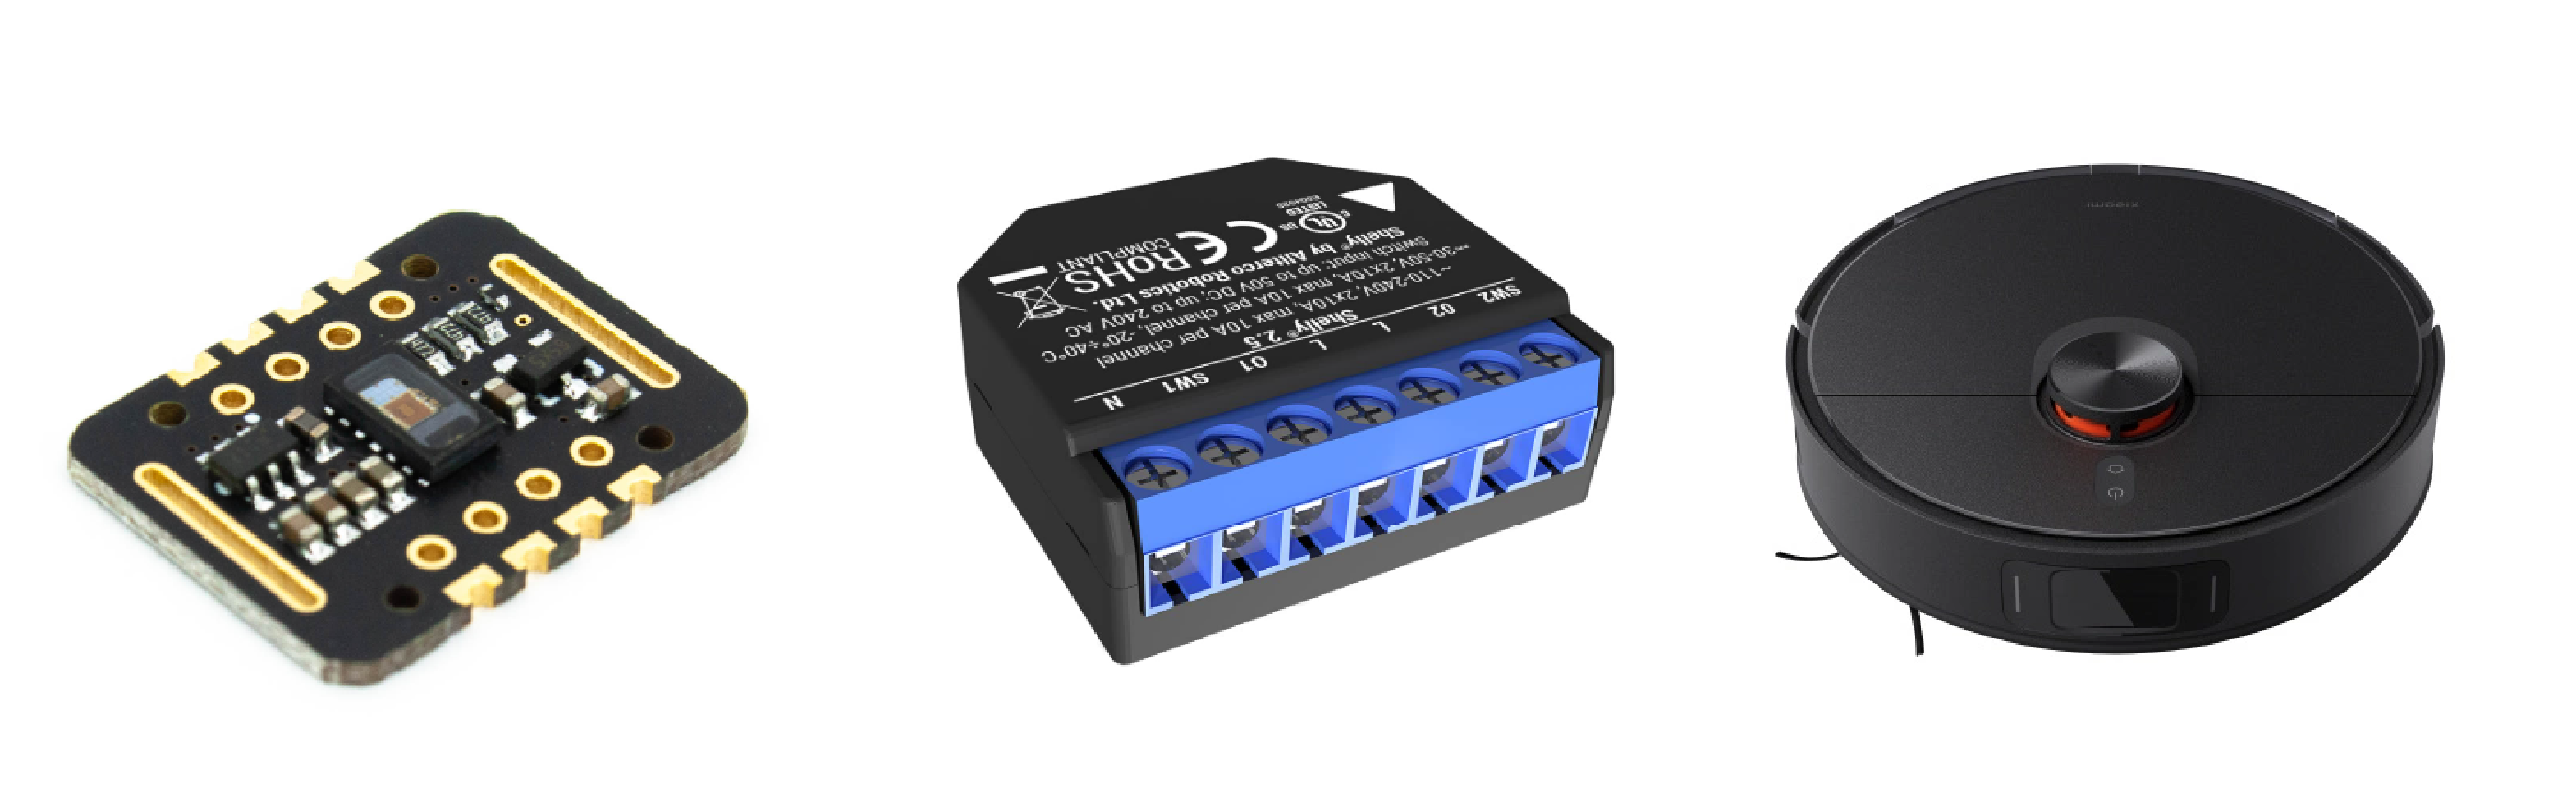
\includegraphics[width=0.8\textwidth]{pictures/urzadzenia-iot.png}
    \caption{Przykładowy sensor, aktuator i urządzenie hybrydowe}
    \label{fig:Przykładowy sensor, aktuator i urządzenie hybrydowe}
\end{figure}

\section{Architektury systemów IoT i ich implikacje bezpieczeństwa}

W systemach IoT wyróżnia się kilka architektur, które mają różne zalety i wady, zwłaszcza pod kątem bezpieczeństwa. Każda z tych architektur wprowadza unikalne wyzwania, które mogą wpływać na stabilność, prywatność i integralność danych. Ogólna architektura IoT przedstawiona jest na rysunku \ref{fig:Ogólna architektura IoT}.

\begin{figure}[h]
    \centering
    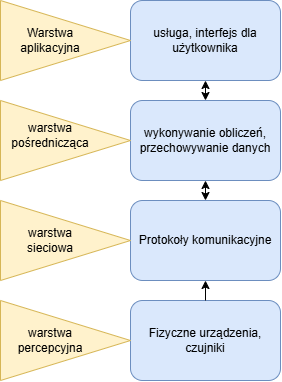
\includegraphics[width=0.3\textwidth]{pictures/IoTarch.drawio.png}
    \caption{Ogólna architektura IoT}
    \label{fig:Ogólna architektura IoT}
\end{figure}

\textbf{3-warstwowa architektura:}
Jest to podstawowy model IoT, który dzieli system na trzy główne warstwy: percepcyjną (obejmuje czujniki, urządzenia aktorów i inne komponenty zbierające dane), sieciową (odpowiada za przesył danych np. Wi-Fi, Bluetooth, LoRaWAN, 5G) i aplikacyjną (przetwarza dane i zapewnia interfejs użytkownikowi). Chociaż model ten jest prosty w implementacji, stanowi cel ataków typu Man-in-the-Middle (atakujący może przechwycić dane) w warstwie sieciowej oraz ataków na interfejsy użytkownika (np. SQL Injection) w warstwie aplikacyjnej. Ataki te mogą prowadzić do przechwycenia lub manipulacji danymi, a także przejęcia kontroli nad systemem.

\textbf{Architektura Edge Computing:}
W tej architekturze przetwarzanie danych odbywa się bezpośrednio na urządzeniach brzegowych (np. inteligentnych kamerach, sterownikach PLC), co pozwala na minimalizację opóźnień. Choć jest to ogromna zaleta, wprowadza również wyzwania związane z fizycznym bezpieczeństwem urządzeń. Ataki fizyczne, takie jak manipulacja urządzeniami lub ich fizyczne usunięcie, mogą być szczególnie groźne. Dodatkowo, ze względu na ograniczone zasoby urządzeń brzegowych, często stosuje się lekkie protokoły komunikacyjne, co może zwiększyć ryzyko ataków \cite{Lynn2020}.

\textbf{Architektura Fog Computing:}
Fog Computing stanowi pomost między urządzeniami brzegowymi (Edge) a chmurą, z wykorzystaniem węzłów przetwarzających dane lokalnie (Fog Nodes). Choć poprawia to wydajność, wprowadza nowe zagrożenia, takie jak ataki typu DDoS na węzły przetwarzające oraz problemy z zarządzaniem tożsamościami w rozproszonym środowisku \cite{Lynn2020}. W szczególności, bezpieczeństwo zarządzania tożsamością i dostępem w tej architekturze stanowi jedno z kluczowych wyzwań, szczególnie w kontekście dużych, heterogenicznych systemów \cite{OpenFog2018}.

\textbf{5-warstwowa architektura:}
Jest to rozwinięcie modelu 3-warstwowego o dodatkowe warstwy: przetwarzania (Edge/Fog Computing) oraz warstwę biznesową. Wprowadza to nowe możliwości, ale także dodatkowe wektory ataku. Przetwarzanie danych na brzegu sieci zmniejsza opóźnienia, ale wymaga odpowiednich zabezpieczeń rozproszonych węzłów przetwarzających. Warstwa biznesowa, odpowiedzialna za analizę danych oraz podejmowanie decyzji, narażona jest na ryzyko wycieku wrażliwych danych, co szczególnie dotyczy systemów, które muszą być zgodne z regulacjami, takimi jak RODO \cite{rao2023iot}.

\textbf{Architektura Cloud-Centric:}
W tej architekturze całość przetwarzania danych odbywa się w chmurze publicznej, co umożliwia dostęp do zaawansowanych narzędzi analitycznych i dużej mocy obliczeniowej. Jednak ta centralizacja danych wiąże się z ryzykiem, zwłaszcza w przypadku nieprawidłowo skonfigurowanych zasobów. Dodatkowo, ograniczenia konkretnego dostawcy chmurowego mogą ograniczyć elastyczność systemu i uniemożliwić łatwą migrację do innych platform.

\textbf{Architektura Peer-to-Peer (P2P):}
Architektura P2P eliminuje pośrednictwo chmury, zapewniając bezpośrednią komunikację między urządzeniami. Dzięki temu użytkownicy zyskują większą prywatność, ponieważ dane nie są przechowywane w centralnych zasobach. Niemniej jednak, brak centralnej kontroli utrudnia implementację skutecznych mechanizmów uwierzytelniania i audytu. Ponadto, w tej architekturze istnieje ryzyko ataków typu Sybil oraz manipulacji danymi, szczególnie w sieciach o niskim poziomie zaufania. Architektura P2P sprawdza się szczególnie w zastosowaniach wymagających niskich opóźnień, takich jak komunikacja między pojazdami.

Szczegółowe porównanie omówionych architektur pod kątem ich cech, zagrożeń i rozwiązań bezpieczeństwa prezentuje tabela \ref{tab:iot_architectures}.

\begin{landscape}
\renewcommand{\arraystretch}{1.5}
\begin{table}[h]
\centering
\caption{Porównanie architektur IoT pod kątem bezpieczeństwa}
\label{tab:iot_architectures}
\begin{tabular}{|l|l|l|l|}
\hline
\textbf{Architektura} & \textbf{Kluczowe cechy} & \textbf{Główne zagrożenia} & \textbf{Rozwiązania bezpieczeństwa} \\ \hline
3-warstwowa & 
\begin{tabular}[c]{@{}l@{}}- Percepcyjna\\ - Sieciowa\\ - Aplikacyjna\end{tabular} &
\begin{tabular}[c]{@{}l@{}}- MITM\\ - Ataki na interfejs\\ - Brak szyfrowania\end{tabular} &
\begin{tabular}[c]{@{}l@{}}- TLS\\ - Uwierzytelnianie MFA\end{tabular} \\ \hline

Edge Computing & 
\begin{tabular}[c]{@{}l@{}}- Przetwarzanie na brzegu\\ - Niskie opóźnienia\end{tabular} &
\begin{tabular}[c]{@{}l@{}}- Ataki fizyczne\\ - Ograniczone zasoby\\ - Ataki na firmware\end{tabular} &
\begin{tabular}[c]{@{}l@{}}- TPM\\ - Aktualizacje firmware\end{tabular} \\ \hline

Fog Computing & 
\begin{tabular}[c]{@{}l@{}}- Węzły przetwarzające\\ - Pośrednia warstwa\end{tabular} &
\begin{tabular}[c]{@{}l@{}}- DDoS\\ - Problemy z tożsamością\end{tabular} &
\begin{tabular}[c]{@{}l@{}}- Blockchain\\ - Detekcja anomalii\end{tabular} \\ \hline

5-warstwowa & 
\begin{tabular}[c]{@{}l@{}}- Dodana warstwa\\ przetwarzania i biznesowa\end{tabular} &
\begin{tabular}[c]{@{}l@{}}- Wyciek danych\\ - Ataki na węzły\end{tabular} &
\begin{tabular}[c]{@{}l@{}}- Szyfrowanie E2E\\ - RBAC\end{tabular} \\ \hline

Cloud-Centric & 
\begin{tabular}[c]{@{}l@{}}- Przetwarzanie w chmurze\\ - Duża moc obliczeniowa\end{tabular} &
\begin{tabular}[c]{@{}l@{}}- Błędy konfiguracji\\ - Vendor lock-in\end{tabular} &
\begin{tabular}[c]{@{}l@{}}- CSPM\\ - Multi-cloud\end{tabular} \\ \hline

Peer-to-Peer & 
\begin{tabular}[c]{@{}l@{}}- Bezpośrednia komunikacja\\ - Wysoka prywatność\end{tabular} &
\begin{tabular}[c]{@{}l@{}}- Ataki Sybil\\ - Brak audytu\end{tabular} &
\begin{tabular}[c]{@{}l@{}}- Mechanizmy reputacji\\ - Blockchain\end{tabular} \\ \hline
\label{tab:architektury-iot}
\end{tabular}
\end{table}
\end{landscape}
\section{Wprowadzenie do zagrożeń w systemach IoT}
Internet Rzeczy (IoT) niesie za sobą wiele korzyści, jednak dynamiczny rozwój tej technologii wiąże się także z licznymi zagrożeniami dla bezpieczeństwa i prywatności użytkowników. Ataki na urządzenia IoT mogą prowadzić do kradzieży danych, zakłóceń w działaniu systemów, a nawet fizycznych uszkodzeń infrastruktury. Poniżej przedstawiono najważniejsze zagrożenia związane z IoT.
\vspace{10pt} \\
\textbf{1. Nieautoryzowany dostęp} do urządzeń IoT to jedno z najczęściej występujących i najgroźniejszych zagrożeń w tym ekosystemie. Głównym powodem tej podatności jest fakt, że wiele urządzeń IoT jest dostarczanych z domyślnymi danymi logowania (np. „admin/admin”), które użytkownicy rzadko zmieniają. Co więcej, część producentów nie umożliwia nawet łatwej zmiany danych uwierzytelniających, co znacznie utrudnia zabezpieczenie tych urządzeń. Taka sytuacja sprzyja atakom typu brute-force, a także wykorzystaniu wcześniej wyciekłych danych logowania dostępnych w sieci.

Atak typu \textbf{brute force (siłowy)} polega na systematycznym próbowaniu wszystkich możliwych kombinacji nazw użytkowników i haseł, aż do momentu uzyskania poprawnych danych logowania. Jest to jeden z najprostszych, ale nadal skutecznych typów ataków, szczególnie w środowisku IoT.

Nieautoryzowany dostęp może mieć poważne skutki w różnych kontekstach środowisk domowych, przemysłowych lub medycynie. W środowiskach domowych, cyberprzestępcy mogą przejąć kontrolę nad inteligentnymi zamkami, systemami alarmowymi, kamerami monitoringu, termostatami czy asystentami głosowymi. Prowadzi to nie tylko do utraty prywatności, ale również może umożliwić fizyczne włamanie do domu bez śladów. W zastosowaniach przemysłowych przejęcie kontroli nad urządzeniami może prowadzić do sabotażu produkcji, awarii maszyn, błędów pomiarowych, a nawet stanowić zagrożenie dla życia pracowników. Szczególnie narażone są systemy SCADA, które często komunikują się bez odpowiedniego szyfrowania i uwierzytelniania. W medycynie nieautoryzowany dostęp do urządzeń medycznych (np. pomp infuzyjnych, monitorów EKG) może prowadzić do nieprawidłowego podania leków lub fałszywych odczytów parametrów życiowych, co może bezpośrednio zagrozić życiu pacjentów. \cite{antonakakis2017mirai}
\vspace{10pt} \\
\textbf{2. Śledzenie użytkowników}, urządzenia Internetu Rzeczy są często wyposażone w sensory i moduły komunikacyjne, które zbierają i przekazują dane dotyczące lokalizacji, aktywności fizycznej, nawyków użytkownika, a nawet parametrów zdrowotnych. Choć dane te są wykorzystywane do poprawy komfortu życia, personalizacji usług czy zwiększenia funkcjonalności urządzeń, to w przypadku niewystarczającej ochrony stają się one poważnym zagrożeniem dla prywatności użytkowników. Istnieje kilka sposobów, w jaki sposób może dochodzić do śledzenia:
\begin{itemize}
    \item \textbf{Analiza ruchu sieciowego} - Nawet jeśli dane są szyfrowane, analiza metadanych (częstotliwości połączeń, adresów IP, wzorców komunikacji) może zdradzić lokalizację lub zachowania użytkownika. \textit{Przykład: } Smartwatch regularnie łączy się z siecią Wi-Fi domową, a następnie z siecią biurową – łatwo wywnioskować miejsce zamieszkania i pracy.
    \item \textbf{Przechwytywanie sygnałów radiowych} -  Urządzenia IoT emitują sygnały Bluetooth, Zigbee, Wi-Fi — te mogą zostać przechwycone zdalnie. \textit{Przykład: } napastnik może ustalić obecność konkretnej osoby w danym miejscu, analizując emisję sygnału opaski fitness.
    \item \textbf{Podatności sprzętowe i firmware'owe} - Niektóre urządzenia posiadają luki w oprogramowaniu, które pozwalają na zdalne odczytywanie współrzędnych GPS lub danych z żyroskopów/akcelerometrów. \textit{Przykład: } inteligentny lokalizator samochodu, który przesyła dane bez szyfrowania – każdy z dostępem do sieci może je odczytać.
    \item \textbf{Nieświadoma zgoda użytkownika} - Aplikacje mobilne zbierają dane, których użytkownicy nie są w pełni świadomi (np. historia połączeń Bluetooth, logi z czujników). Dane te są często agregowane, sprzedawane lub przekazywane podmiotom trzecim (np. firmom reklamowym).
\end{itemize}
Skutkami śledzenia może być inwigilacja, stalking cyfrowy, kradzież tożsamości, czy profilowanie behawioralne. Jednym z najbardziej znanych ataków przeprowadzancyh w celu śledzenia użytkowników jest atak Man-in-the-Middle.
\vspace{10pt} \\
\textbf{3. Ataki typu Man-in-the-Middle (MITM)} polega na przechwyceniu i ewentualnej modyfikacji danych wymienianych pomiędzy dwoma stronami komunikacji — np. między urządzeniem IoT a serwerem w chmurze lub aplikacją mobilną użytkownika. W klasycznym scenariuszu atakujący „podszywa się” jednocześnie pod obie strony, nie ujawniając swojej obecności. W kontekście Internetu Rzeczy MITM jest szczególnie groźny, ponieważ wiele urządzeń korzysta z uproszczonych, lekkich protokołów komunikacyjnych, nie wdraża domyślnie szyfrowania (lub robi to w sposób nieprawidłowy), często działa na otwartych lub słabo zabezpieczonych środowiskach. W pierwszej fazie takiego ataku napastnik uzyskuje dostęp do sieci, w której znajduje się urządzenie IoT (np. poprzez niezabezpieczone Wi-Fi), po czym ustawia swoje urządzenie jako pośrednik między ofiarą a serwerem. Następnie jeśli komunikacja nie jest szyfrowana, dane mogą być przechwycone „w czystej postaci” (np. loginy, hasła, dane lokalizacyjne). Możliwa jest także manipulacja danymi w locie — np. zmiana polecenia sterującego lub wartości z czujnika. Schemat działania tego ataku w kontekście inteligentnego domu zobrazowano na rysunku \ref{fig:Schemat ataku typu Man-in-the-Middle (MITM) w systemach IoT}.
\begin{figure}[h]
    \centering
    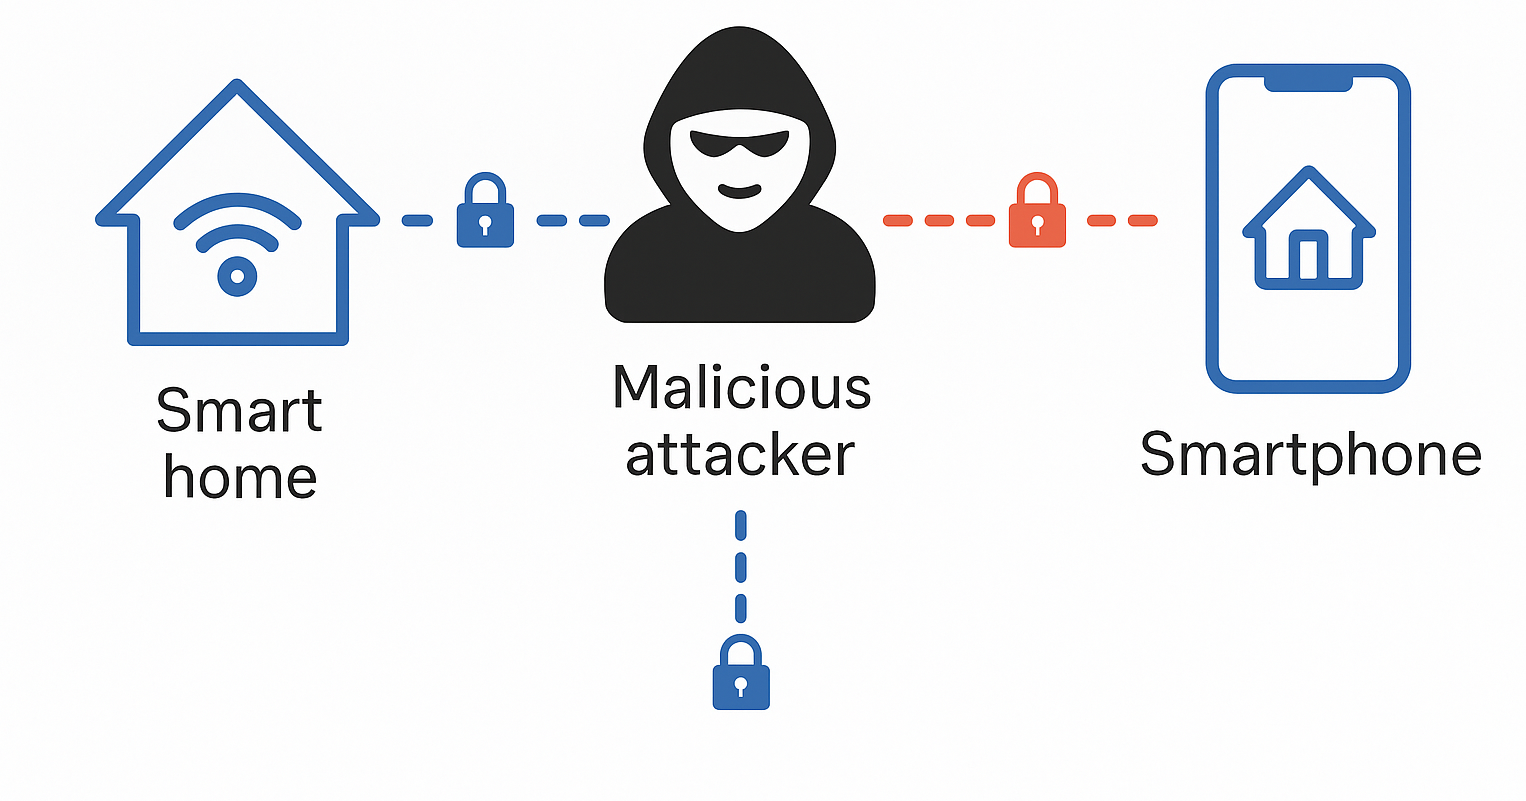
\includegraphics[width=0.6\textwidth]{pictures/MITM.png}
    \caption{Schemat ataku typu Man-in-the-Middle (MITM) w systemach IoT}
    \label{fig:Schemat ataku typu Man-in-the-Middle (MITM) w systemach IoT}
\end{figure}
\vspace{10pt} \\
\textbf{4. Manipulacja danymi} w systemach IoT stanowi jedno z bardziej podstępnych i trudnych do wykrycia zagrożeń, polegające na celowej zmianie, wstrzykiwaniu lub fałszowaniu przesyłanych danych. W przeciwieństwie do ataków ukierunkowanych na zakłócenie działania urządzeń, manipulacja danymi ma na celu wprowadzenie odbiorcy w błąd, co może prowadzić do błędnych decyzji systemów sterujących lub użytkowników.
W praktyce manipulacja danymi może przyjmować wiele form:
\begin{itemize}
    \item \textbf{Fałszowanie pomiarów} - w środowiskach medycznych może to oznaczać zmianę danych zbieranych przez czujniki monitorujące stan zdrowia pacjenta (np. tętno, ciśnienie krwi), co może prowadzić do niewłaściwej diagnozy i zagrożenia życia.
    \item \textbf{Sabotaż procesów przemysłowych} - atakujący mogą zmienić dane z czujników temperatury, ciśnienia lub wilgotności, co może doprowadzić do błędnych decyzji systemów automatyki i uszkodzenia maszyn lub całych linii produkcyjnych.
    \item \textbf{Zakłócenie systemów transportowych} - inteligentne systemy sterujące ruchem, bazujące na danych z wielu źródeł (czujniki, GPS, sygnalizacja), mogą zostać zmanipulowane, co może skutkować wypadkami, korkami lub nieprawidłowym sterowaniem ruchem.
    \item \textbf{Dezinformacja w systemach analitycznych} - manipulacja może dotyczyć np. danych środowiskowych (zanieczyszczenie powietrza, poziom hałasu), co może prowadzić do błędnych wniosków analitycznych i decyzji na poziomie zarządzania miastem.
    \item \textbf{Fałszywe alarmy i sabotaż} - w inteligentnych budynkach lub systemach zabezpieczeń zmiana danych z czujników (np. dymu, ruchu) może prowadzić do nieuzasadnionych alarmów, które dezorganizują pracę instytucji lub przedsiębiorstw.
\end{itemize}
Technicznie manipulacja danych może być przeprowadzona na różnych poziomach: ataki MITM, na poziomie samego urządzenia, na poziomie agregatorów danych, W systemach analitycznych lub bazach danych. Z uwagi na to, że IoT opiera się na automatycznym przetwarzaniu dużych ilości danych, ich integralność jest kluczowa. Nawet niewielka zmiana może spowodować poważne skutki w skali całego systemu \cite{schneier2018}.
\vspace{10pt} \\
\textbf{5. Ataki typu DDoS (Distributed Denial of Service) i DoS (Daniel of Service)} stanowią jedne z najpoważniejszych zagrożeń dla systemów Internetu Rzeczy. Ich celem jest zakłócenie lub całkowite uniemożliwienie działania danej usługi, aplikacji lub urządzenia, co może prowadzić do poważnych strat finansowych, przestojów w działaniu systemów oraz zagrożeń dla bezpieczeństwa użytkowników. 

Atak typu DoS polega na przeprowadzeniu przez jedno źródło (np. jedno urządzenie lub komputer) dużej liczby zapytań do danego systemu, serwera lub aplikacji w krótkim czasie. Celem jest przeciążenie zasobów docelowego systemu – takich jak pamięć, CPU lub pasmo sieciowe – aż do momentu, gdy stanie się on niedostępny dla legalnych użytkowników. Chociaż ataki DoS są relatywnie proste do zrealizowania, ich skuteczność w środowisku IoT jest większa z uwagi na ograniczoną moc obliczeniową i słabe zabezpieczenia wielu urządzeń. Przykład: prosty atak może skutecznie unieruchomić inteligentne czujniki, routery lub bramy IoT wykorzystywane np. w systemach monitoringu lub automatyki domowej.

DDoS to rozwinięcie ataku DoS, w którym udział bierze wiele rozproszonych źródeł – często setki tysięcy zainfekowanych urządzeń IoT. Tworzą one tzw. botnet, czyli sieć zombie – urządzeń zdalnie sterowanych przez atakującego.
Skutkami takich ataków w środowiskach IoT mogą być:
\begin{itemize}
    \item Zakłócenie działania infrastruktury krytycznej, np. systemów transportu, opieki zdrowotnej, automatyki przemysłowej.
    \item Straty finansowe wynikające z przestojów, kar umownych i konieczności przywracania usług.
    \item Utrata zaufania klientów i reputacji marki.
    \item Możliwość wykorzystania jako punktu wyjścia do innych, bardziej zaawansowanych ataków, takich jak manipulacja danymi czy kradzież informacji.
\end{itemize}

Przykładem z życia może być rekordowy atak DDoS w Polsce - W maju 2025 roku CERT Orange Polska odparł największy atak DDoS w historii polskiego internetu. Atak, który trwał kilka dni, osiągnął szczytowy ruch na poziomie 1,3 terabita na sekundę (Tbps). Dla porównania, przeciętne domowe łącze internetowe w Polsce ma przepustowość około 200 megabitów na sekundę (Mbps), co podkreśla skalę tego incydentu. \cite{certorange2025}
\vspace{10pt} \\
\textbf{6. Brak aktualizacji i podatności w oprogramowaniu}, wiele urządzeń IoT działa na oprogramowaniu, które nie jest regularnie aktualizowane, co znacząco zwiększa ryzyko wykorzystania znanych luk bezpieczeństwa. Producenci często nie zapewniają odpowiedniego wsparcia technicznego — w tym poprawek bezpieczeństwa czy aktualizacji systemów operacyjnych i firmware’u — przez co urządzenia pozostają narażone na ataki przez długi czas. Ponadto, nawet jeśli aktualizacje są dostępne, to użytkownicy często nie mają łatwej możliwości ich samodzielnego instalowania lub wręcz nie są świadomi potrzeby regularnej aktualizacji. W wielu przypadkach proces aktualizacji wymaga specjalistycznej wiedzy lub ingerencji serwisu, co powoduje, że aktualizacje są pomijane lub opóźniane. Brak regularnych aktualizacji powoduje, że urządzenia IoT stają się łatwym celem dla cyberprzestępców, którzy mogą wykorzystać istniejące podatności do przejęcia kontroli nad systemami, podsłuchiwania komunikacji, wprowadzania złośliwego oprogramowania lub tworzenia botnetów wykorzystywanych do ataków DDoS i innych działań przestępczych. W praktyce oznacza to, że nawet najnowsze i najbardziej zaawansowane urządzenia mogą stać się zagrożeniem, jeśli ich oprogramowanie nie jest odpowiednio i systematycznie zabezpieczane. W konsekwencji, brak aktualizacji nie tylko naraża prywatność i bezpieczeństwo użytkowników, ale może mieć również poważne skutki dla całej infrastruktury sieciowej \cite{johnston2019}.
\vspace{10pt} \\
\textbf{7. Ataki fizyczne} na urządzenia IoT to realne zagrożenie, szczególnie w przypadku systemów rozmieszczonych w przestrzeni publicznej, przemysłowej lub trudno nadzorowanej. Urządzenia IoT, takie jak czujniki, kamery, bramki komunikacyjne czy sterowniki PLC, często działają w niekontrolowanych środowiskach, co czyni je podatnymi na manipulacje fizyczne. Atakujący mogą uzyskać fizyczny dostęp do urządzenia w celu: zresetowania ustawień do wartości fabrycznych i przejęcia nad nim kontroli, podłączenia interfejsów debugowania (np. UART), aby uzyskać dostęp do firmware'u lub danych, zainstalowania złośliwego oprogramowania, wymiany komponentów elektronicznych lub podmiany całego urządzenia, zasilania urządzenia w celu obserwacji jego działania w bezpiecznym środowisku laboratoryjnym. W sektorach takich jak przemysł, transport czy smart city, skutki takich ataków mogą być poważne — od wycieku danych po sabotaż procesów operacyjnych. Przykładem może być manipulacja czujnikami w inteligentnych systemach sterowania ruchem lub dostęp do lokalnych węzłów sieci energetycznych. 
\vspace{10pt}
Internet Rzeczy wprowadza zasadnicze zmiany w sposobie gromadzenia i przetwarzania danych, jednocześnie tworząc nowe wektory potencjalnych ataków. Ograniczenia sprzętowe wielu urządzeń stanowią poważną barierę w implementacji zaawansowanych mechanizmów ochrony. Choć protokoły komunikacyjne są zoptymalizowane pod kątem wydajności, często okazują się niewystarczające w kontekście zapewnienia odpowiednich zabezpieczeń.